% article example for classicthesis.sty
\documentclass[10pt,a4paper]{article} % KOMA-Script article scrartcl
\usepackage{import}
\usepackage{xifthen}
\usepackage{pdfpages}
\usepackage{transparent}
\newcommand{\incfig}[1]{%
    \def\svgwidth{\columnwidth}
    \import{./figures/}{#1.pdf_tex}
}
\usepackage{lipsum}     %lorem ipsum text
\usepackage{titlesec}   %Section settings
\usepackage{titling}    %Title settings
\usepackage[margin=10em]{geometry}  %Adjusting margins
\usepackage{setspace}
\usepackage{listings}
\usepackage{amsmath}    %Display equations options
\usepackage{amssymb}    %More symbols
\usepackage{xcolor}     %Color settings
\usepackage{pagecolor}
\usepackage{mdframed}
\usepackage[spanish]{babel}
\usepackage[utf8]{inputenc}
\usepackage{longtable}
\usepackage{multicol}
\usepackage{graphicx}
\graphicspath{ {./Images/} }
\setlength{\columnsep}{1cm}

% ====| color de la pagina y del fondo |==== %
\pagecolor{white}
\color{black}



\begin{document}
    %========================{TITLE}====================%
    \title{{  Parcial 1 Álgebra Abstracta  }}
    \author{{Rodrigo Castillo}}
    \date{\today}

    \maketitle


    %=======================NOTES GOES HERE===================%
    \section{ Punto 1 }
        \begin{figure}[h!]
            \centering
            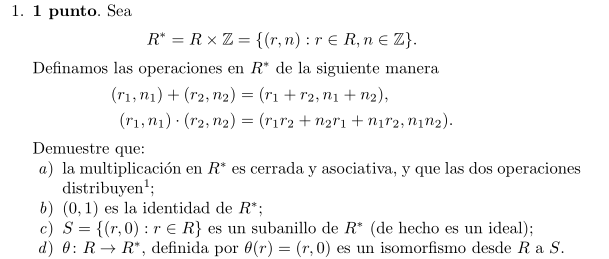
\includegraphics[width=0.8\linewidth]{punto1.png}
            \caption{Punto 1}
            \label{punto1}
        \end{figure}

        \subsection{a}

            \subsubsection{la multiplicacion es cerrada y asociativa}
                demostración :
                \\
                sean $ (x_1 , m_1 ) , (x_2 , m_2 ) \in R*  $  , por lo tanto  $
                (x_1,m_1)(x_2 , m_2) = (x_1x_2 + x_1m_2 + x_2m_1 , m_1m_2)  $
                \\
                note que $ x_1,x_2 \in R  $ y que $ m_1 , m_2 \in Z  $ , por lo tanto, tenemos que
                \\
                $ x_1x_2 \in R  $  , $ x_1m_2 \in R  $  , $ x_2m_1 \in  R  $ , $
                m_1m_2 \in Z  $ , luego $ (x_1x_2 + x_1m_2 + x_2m_1) \in R
                $ y $ (m_1m_2) \in Z  $ , como así lo definimos, entonces tenemos que ...
                \\
                $ (x_1,m_1)(x_2,m_2) \in R \times Z  $
                \\
                $ (x_1,m_1)(x_2,m_2) \in R* $
                \\
                como $ (x_1 , m_1) , (x_2 ,m_2)   $ son elementos cualesquiera de $
                R*  $ , entonces tenemos que para cualquier elementos en $ R*  $ ,
                la multiplicación es cerrada

            \subsubsection{la suma distribuye}
                sean $ (x_1,m_1),(x_2,m_2)(x_3  , m_3) \in R  $ , por lo tanto

                $ ((x_1, m_2) + (x_2 , m_2)) + (x_3 , m_3 )= (x_1 + x_2 , m_1 +
                m_2)+(x_3,m_3)  $
                 \\
                 $ = (x_1 + x_2 + x_3 , m_1 + m_2 + m_3 )
      $              \\
                 $ =( x_1 + (x_2 + x_3) , m_1 + (m_2 + m_3))  $
                 \\
                 $ =(x_1 , m_1) + (x_2 + x_3 , m_2 + m_3)  $
                 \\
                 $ =(x_1 , m_1) + ((x_2,m_2) + (x_3 , m_3))  $
                 \\
                 por lo tanto la suma distribuye en $ R*  $

             \subsubsection{la multiplicación distribuye en $ R*  $ }
                demostración :
                \\
                sean $ (x_1,m_1),(x_2,m_2)(x_3  , m_3) \in R  $ , por lo tanto
                \\
                $ ((x_1 ,m_1)(x_2,m_2))(x_3 , m_3)  = (x_1x_2 + m_2x_1 + m_1x_2 , m_1m_2)(x_3 , m_3) $
                \\
                $ = (x_1x_2x_3 + m_3m_2x_1 + x_3x_2m_2 , m_3m_2m_1)  $
                \\
                $ = (x_1(x_2x_3) + (m_3m_2)x_1 + (x_3x_2)m_2 , (m_3m_2)m_1)  $
                \\
                $ = (x_1,m_1)((x_2,m_2)(x_3,m_3))  $
                \\
                por lo tanto el producto distribuye en $ R*  $


                \subsection{ $ (0,1)  $  es la identidad de $ R  $  }
            demostración:
            \\
            sea $ (x_1 , m_1)  $  un elemento arbitrario de $ R*  $  , por lo tanto ...
            \\
            $ (0,1)(x_1,m_1) = (x_1 \cdot 0 + 1 \cdot x_1 + 0 \cdot m_1 , 1 \cdot m_1) $
            \\
            $ = (0 + x_1 + 0  , m_1 )  $
            \\
            $ =(x_1,m_1)  $
            \\
            acá podemos ver que se cumple que es identidad en este sentido, ahora
            procederemos a ver que es identidad en el otro sentido también :
            \\
            $ (x_1 , m_1 ) \cdot (0 ,1 ) = (x_1 \cdot 0 + 1 \cdot x_1  + 0 \cdot m_1  , 1 \cdot m_1)  $
            \\
            $ = (x_1,m_1)  $
            \\
            como se cumple en ambos sentidos, entonces tenemos que $ (0,1) \in
            R*  $ es una identidad.


            \subsection{$ \theta : R \to R*  $ definida como $ \theta (x) =
            (x,0)  $ es un subanillo de $ R*  $ }
                \subsubsection{cerrado bajo la multiplicación}
                    sean $ (x_1 , 0) , (x_1 ,0) \in R*  $ , por lo tanto...
                    \\
                    $ (x_1,0) \cdot (x_2,0) = (x_1x_2 + 0 + 0 , 0 )  $
                    \\
                    $ = (x_1x_2 , 0 )  $
                    \\
                    note que $ x_1 , x_2 \in R  $ , por lo tanto $ (x_1x_2 , 0)
                     $ está en el subanillo, luego la multiplicación es cerrada .
                \subsubsection{la resta es cerrada}
                    sean $ (x_1 , 0) , (x_1 ,0) \in R*  $ , por lo tanto...
                    \\
                    $ (x_1 ,0) - (x_2 , 0) = (x_1 - x_2 , 0 -0 )  $
                    \\
                    $ = (x_1 -x_2 , 0)  $
                    \\
                    note que $ x_1-x_2 \in R  $ , luego  $ (x_1 -x_2 , 0)  $
                    está en el subanillo ,  luego la resta también es cerrada.

            \subsection{$ \theta : R \to R*   $ definida por $
            \theta(x) = (x,0)  $  es un isomorfismo de $ R  $ a $ S  $}
                \subsubsection{es un homomorfismo :}
                    \begin{itemize}
                        \item {
                                sean $ x , y \in R  $  , luego $ \theta (x+y) = (x+y,0)  $
                                \\
                                mientras que $ \theta (x) + \theta (y) = (x,0)
                                + (y,0) = (x+y , 0+0) = (x+y,0)  $
                                \\
                                luego $ \theta (x) + \theta (y) = \theta (x+y) = (x+y,0)  $
                            }
                        \item {
                                sean $ x , y \in R  $  , luego $ \theta(xy)  = (xy,0)  $
                                \\
                                mientras que $ \theta(x) \theta(y) = (x,0)\cdot (y,0)  $
                                \\
                                $ = (xy + 0 + 0 , 0 )  $
                                \\
                                $ = (xy,0)  $
                                \\
                                luego $ \theta (x) \theta (y) = \theta (xy) = (xy,0)  $
                            }
                    \end{itemize}
                \subsubsection{es sobreyectivo}
                    debo probar que para todo $ x \in R  $ existe un $ y \in R*  $ tal que $ \theta (x) = y  $ :
                    \\
                    demostración:
                    \\
                    sea $ y \in R* = (x , 0)  $  , tenemos que para cualquier $
                    x  $ arbitrario en $ R  $  se tiene que $ \theta (x) =
                    (x,0) = y  $ .
                \subsubsection{es inyectivo}
                    debo probar que si $ \theta (x) = \theta (y) \Rightarrow x = y  $
                    \\
                    demostración por contrarrecíproca:
                    \\
                    supongamos que $ x \not= y   $  , por lo tanto $ (x,0) \not= (y,0)  $
                    \\
                    note que $ \theta (x) = (x,0)  $
                    \\
                    note que $ \theta (y) = (y,0)  $
                    \\
                    por lo que , por transitividad tenemos que $ \theta (x) \not=
                    \theta (y)  $

                \subsubsection{conclusión}
                    como existe un homomorfismo y la transformación es
                    biyectiva, entonces es un isomorfismo de $ R \to S  $


    \section{Sea $ \theta R \to S  $  un homomorfismo de anillos Demuestre }

        \subsection{si $ R  $ es conmutativo entonces $ \theta (R)  $ es
        conmutativo}

            demostración:
            \\
            Supongamos que $ R  $ es un anillo conmutativo, es decir que para
            todo $ x,y \in R  $  se tiene que $ (xy) = (yx)  $ .
            \\
            por lo tanto $ \theta (xy) = \theta (yx)  $
            \\
            como $ \theta   $ es un homomorfismo entonces tengo que $ \theta
            (xy)  = \theta (x) \theta (y) $
            \\
            y similarmente tengo que $ \theta (yx) = \theta(y) + \theta (x)   $
            \\
            pero note que $ \theta (xy) = \theta (yx)  $  , luego por
            transitividad se tiene que $ \theta (x) \theta (y) = \theta (y)
            \theta (x) $ , luego $ \theta (R)  $  es conmutativo .

        \subsection{ si $ R  $ tiene elemento identidad 1 , $ S \not= 0  $
            y $   \theta $ es sobreyectiva entonces $ \theta (1)  $  es la identidad
            de $ S  $  }

            demostración por contradicción :
            \\
            supongamos que $ R  $ tiene elemento identidad 1 , $ S \not= 0
            $  y $ \theta   $ es sobreyectiva pero $ \theta (1)  $ no es la
            identidad .
            \\
            sea $ s \in R  $ , como $ R  $ tiene elemento identidad $ 1  $
            entonces $ \theta (s \cdot 1)  \in S $  . note que , $ \theta   $
            es un homomorfismo, por lo que  $ \theta (1 \cdot s) = \theta
            (1) \cdot \theta (s)  $ y además note que $ \theta  $ es sobreyectiva .
            \\
            luego $ \theta (1 \cdot s)  $
            \\
            $ = \theta (1) \theta (s)  $
            \\
            $ = \theta (s)  $
            \\
            sin embargo supusimos que $ 1  $ no es la identidad de $ S  $ , luego
            \\
            $ \theta(1) \cdot \theta(s) \not= \theta(s)  $
            \\
            luego tenemos que $ \theta (s) \not= \theta (s)  $  , y esto es
            una contradicción clara.

        \subsection{Punto B}
        \subsection{Punto C}


    \section{Punto 3}
        \begin{figure}[h!]
            \centering
            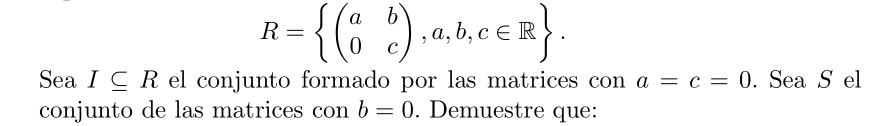
\includegraphics[width=0.8\linewidth]{punto2.png}
            \caption{Punto 3 enunciado}
            \label{fig}
        \end{figure}

        Definimos $ I  $
        \begin{equation}
            I = \begin{pmatrix}
                0 & b
                \\
                0 & 0
            \end{pmatrix}
            \\
             , b \in R
        \end{equation}
        \\
        Definimos $ S  $
        \begin{equation}
            S = \begin{pmatrix}
                a & 0
                \\
                0 & c
            \end{pmatrix}
        \end{equation}

        \subsection{Es $ I  $ un ideal de $ R  $  ?}
            Demostración , sea $ A \in R  $  y $ B \in I  $  , por lo tanto $ A
            \cdot B  =  $
            \begin{equation}
                A \cdot  B = \begin{pmatrix}
                    a & b
                    \\
                    0 & c
                \end{pmatrix}
                \cdot
                \begin{pmatrix}
                    0 & b
                    \\
                    0 & 0
                \end{pmatrix}
            \end{equation}
            solucionando esta multiplicación tenemos que
            \begin{equation}
                A \cdot B = \begin{pmatrix}
                    (a \cdot 0) + (b \cdot 0) & (a \cdot b )+ (b ^{2} )
                    \\
                    (0 \cdot 0)+(c \cdot 0) & (0- \cdot b) + (0 \cdot 0)
                \end{pmatrix} =
                \begin{pmatrix}
                    0 & (b ^{2} + ab)
                    \\
                    0 & 0
                \end{pmatrix}
            \end{equation}
            note que el polinomio $ (b ^{2}  + ab)  \in R $ , por lo tanto $ A \cdot B \in I
            $ , luego $ I  $ es un ideal de $ R  $

        \subsection{S es un subanillo de $ R  $   , es un ideal?}
            \subsubsection{S es un subanillo de R}
                demostración para la Multiplicación ...
                \\
                sean $ A \in S  $  y $ B \in S  $ , luego tenemos que
                \begin{equation}
                    A \cdot B = \begin{pmatrix}
                        a & 0
                        \\
                        0 & c
                    \end{pmatrix}
                    \cdot \begin{pmatrix}
                        a & 0
                        \\
                        0 & c
                    \end{pmatrix}
                    =
                    \begin{pmatrix}
                        a ^{2} & (a \cdot 0) + (0 \cdot c)
                        \\
                        (0 \cdot a) + (0 \cdot c) & c ^{2}
                    \end{pmatrix}
                \end{equation}
                \begin{equation}
                     = \begin{pmatrix}
                        a ^{2} & 0
                        \\
                        0 & c ^{2}
                    \end{pmatrix}
                    = C
                \end{equation}
                como $ a ^{2} , c^{2} \in R    $ tengo que la multiplicación es
                cerrada pues $ C \in S  $
                \\
                Demostración para la resta ...
                \\
                Sean $ A_1 \in S , B_2 \in S  $ , por lo tanto
                \begin{equation}
                    A = \begin{pmatrix}
                        a_1  & 0
                        \\
                        0 & c_1
                    \end{pmatrix}
                \end{equation}
                \begin{equation}
                    A_2 = \begin{pmatrix}
                        a_2 & 0
                        \\
                        0 & c_2
                    \end{pmatrix}
                \end{equation}
                por lo tanto $ A_1 - A_2  $  se define como
                \begin{equation}
                    C = \begin{pmatrix}
                        a_1 - a_2 & 0
                        \\
                        0 & c_1 - c_2
                    \end{pmatrix}
                \end{equation}
                note que $ C \in S  $ , luego , al cumplir la cerradura de la
                resta y de la multiplicación, se tiene que $ S  $ es un
                subanillo de $ R  $

            \subsubsection{S es un ideal para R?}
                no es un ideal...
                \\
                prueba: Sea $ A \in  R  $  y $ B \in  S  $ , al multiplicar $ A
                \cdot  B  $  obtengo la siguiente matrix
                \begin{equation}
                    A \cdot  B = \begin{pmatrix}
                        a ^{2} & bc
                        \\
                        0 & c ^{2}
                    \end{pmatrix}
                    = C
                \end{equation}
                note que el elemento $ C_{12} \not= 0  $ si $ b , c \not= 0  $
                , luego la matriz $ C  $ no pertenece al subanillo $ S  $ ,
                luego no es un ideal de $ S  $

        \subsection{c}





































    %=======================NOTES ENDS HERE===================%

    % bib stuff
    \nocite{*}
    \addtocontents{toc}{{}}
    \addcontentsline{toc}{section}{\refname}
    \bibliographystyle{plain}
    \bibliography{../Bibliography}
\end{document}
